\chapter{Deep Reinforcement Learning}
Deep Learning describes a family of learning techniques
that at their core are about learning representations of data
in a hierarchical fashion.
It replaces the need for handcrafted feature
and indeed works in an entirely unsupervised or at least
semi-supervised fashion.
In this way,
it is often deployed as end-to-end learning
because it can learn its own higher-level abstractions
from raw data.

The core algorithm in deep learning is backpropagation
(described in detail in \ref{sec:backprop})
which describes how a learning model should update its parameters
in response to a discrepancy between learned output
and example output.

\paragraph{}
While the notion of stacking layers of units
to create multi-tiered artificial neural networks
has been around for a few decades already,
the recent surge in computing power
has enabled these conceptual models
to be actually built large enough
to explore their full potential.

Next to fully connected neural networks,
there are a few other types of networks of interest
that I will explore.
One such is the Convolutional Neural Network
which I will describe in more detail in
section \ref{sec:cnn}.
This type especially has benefitted from
advances in technology because of their highly
parallel nature which effectively allows them to be run
on consumer graphic hardware which is ever-improving
and becoming more accessible.

\paragraph{}
The areas that have benefited most from
this branch of machine learning
include without doubt
image recognition and speech recognition,
both problems with extremely noisy real-world data
that were typically tackled
by hand-crafting higher level features
and learning from those,
yet it is far from limited to these.
Deep learning has been extensively and successfully
applied to reinforcement learning as well,
the main topic of interest in this thesis.

\paragraph{}
The rest of this chapter will start by introducing
core deep learning concepts,
then proceed to applying deep learning
to the reinforcement learning case.
Sections \ref{sec:cnn} and \ref{sec:rnn}
concern themselves with general deep learning techniques,
i.e. not specific to the reinforcement learning.
Section \ref{sec:dqn}
explores the Deep Q-Network architecture
which forms the basis for the rest of this thesis.

\section{Convolutional Neural Networks}
\label{sec:cnn}
The core to deep learning is that representations
of data can be learned in an unsupervised
or semi-supervised manner
without the need for handcrafted features.
Convolutional networks are able to learn features
from raw input without any human intervention.
Stacking convolutional layers even allows
hierarchical features to be learned.
This way the initial layer could function
as an edge detector
whereas deeper layers
would learn higher-level abstractions
such as for example facial features
in the case of image recognition.

Another core property of convolutional layers is that,
unlike a regular fully connected neural network,
it can recognize the same features
regardless of the location of the feature in the input.
A regular fully connected network would need to have
its weights in each of the possible locations trained to recognize the same feature
which is wasteful in both space and computational requirements.

\paragraph{}
Convolutional networks are strongly inspired
by the animal visual cortex which contains two basic cell types.
Simple cells activate respond most strongly to edge patterns;
they function as edge-detectors and have a small receptive field.
Complex cells on the other hands have a larger receptive field
and are also spatially invariant to pattern location.

An early predecessor of the convolutional network
that tried to capture these concepts
is the neocognitron
\parencite{Fukushima1980}
which differs mostly in that convolutional networks
share weights across several positions in the input,
as I will explain further down.
The architecture I will explain in the following section
is based on the famous LeNet-5,
designed by
\citeauthor{LeCun1998}
(\citeyear{LeCun1998})
to successfully recognize hand-written letters.

\section{Building Blocks}
\label{sec:building_blocks}

\subsection{Convolutional Layer}
The core building block for a convolutional network
is the convolutional layer.
For the remainder of this text it is easiest
to think of input as images, possibly
with a depth dimension (such as color).

\begin{figure}[htpb]
  \centering
  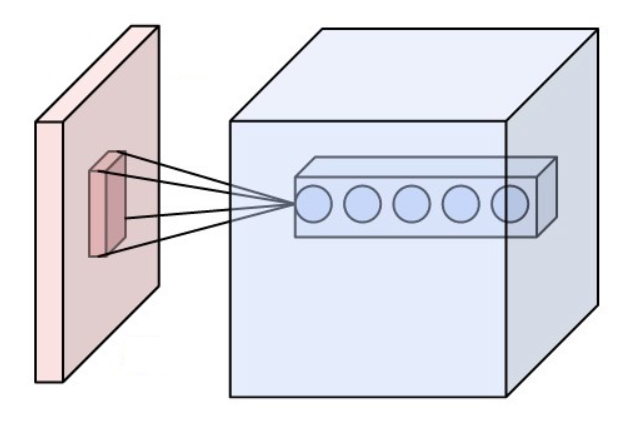
\includegraphics[width=0.7\linewidth]{conv_layer.png}
  \caption[Convolutional layer]{Convolutional layer (blue) connected to an input layer.
    Highlighted are multiple filters connecting to a single input tile.
  }
  \label{fig:conv_layer}
\end{figure}

\paragraph{}
Let us start with the notion of a single, trainable neuron
in the convolutional layer.
It connects to only a small part of
the underlying input layer
as demonstrated in
Figure \ref{fig:conv_layer},
albeit through the whole depth.
This is the receptive field
as I described earlier.
Strongly connecting to only a small part of the input
is what allows convolutional networks
to exploit strong local correlations
that are inherently present
in natural images
but also in many other forms of
naturally occurring data.

\paragraph{}
This single neuron is part of a filter
that spans the whole input image,
it has neighbors that just like it
fully connect to neighboring patches of input.
One such a filter is now a flat 2D activation map
for a single feature.
This replication for a single filter
is what makes convolutional networks
insensitive to the location of a feature.

Of course we would like to have multiple features,
so we stack multiple of these filters on top of one another.
This stacking behavior of filters is described in
Figure \ref{fig:conv_layer},
where a single input patch is shown to correspond
to several filters.

\subsection{Parameter Sharing}
\label{sub:parameter_sharing}
As stated before, one feature corresponds to neurons across
the whole input by each corresponding to some patch of it.
This relies on the assumption that the feature could arise
anywhere in the input and would be useful to discover anywhere.
In order to actually compute the same feature,
we constrain the weights and bias of the neurons for a single feature
to be shared.

\subsection{Details}
\label{sub:details}
To actually generate the feature map
we \textit{convolve} the input with a linear filter,
add a bias and afterwards apply a non-linear function
such as a rectifier
(described in Section \ref{sec:relu}).
It is only because the weights are shared across a single feature
that this convolution is possible,
hence the name of the layer.

\paragraph{}
A single feature map $k$ in terms of its input $x$ could be computed as:

\begin{equation}
  h_k = tanh((W_k \cdot x) + b_k)
\end{equation}

It is also this operation that allows convolutional networks
to run so efficiently on parallel hardware,
making it the ideal candidate
for general purpose GPU computing.

\subsection{Tuning}
A single convolutional layer
has some hyperparameters that are both important
and hard to tweak.
Since learning a convolutional network
is still a rather slow endeavour,
it is best to start out with good estimates from the deep learning community.

\paragraph{}
The common way to build a convolutional network
from convolutional layers is to have
the layers closer to the input compute
few features,
computed over large receptive fields or tiles.
As the network grows deeper,
inputs to layers represent higher level features
and can thus be learned from smaller input tiles;
intuitively, a few high-level features
can contain the same information of more
lower-level features.
Conversely, while there are only few
worthwhile raw features such as different types of edges,
there are probably more distinct higher-level features
that can be used to generate the final output.
Deeper layers should thus grow deeper yet slimmer spatially.

This setup typically results in a funnel-like structure
such as shown in Figure \ref{fig:conv_layer_funnel}.
The deepening occurs because of the increase in features
whereas the slimming usually occurs because multiple
outputs from an input layer correspond to only a single
neuron, spatially, in the next layer.
However, there are ways to train a neuron on a patch of input
yet still retain output size (again, spatially).
These I will describe below.

\begin{figure}[htpb]
  \centering
  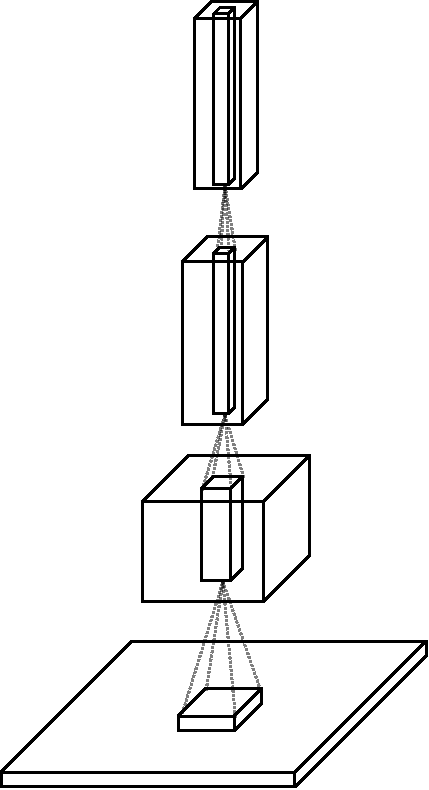
\includegraphics[angle=90,width=0.7\linewidth]{conv_funnel.pdf}
  \caption[Convolutional layers stacked]{
    Convolutional layers can be stacked
    in a funnel-like manner (right to left),
    growing smaller spatially
    yet larger in the depth or feature dimension.
  }
  \label{fig:conv_layer_funnel}
\end{figure}

\paragraph{}
As noted, both the amount of features
as well as the size of the receptive field in a layer
play a huge role in the representational capacity of the layer.
Still, there are other ways to affect this.
\begin{description}
  \item[Stride]
    The stride for a convolutional layer determines the spacing
    between receptive fields, or tiles.
    A stride of 1 would have very strongly overlapping tiles
    and as a result larger spatial dimensions
    than a lower stride would have.
    A stride equal to the tile size
    would result in non-overlapping but touching tiles.
    An even larger one would, of course,
    result in unused input elements and is therefore
    rather unpopular in practice.
  \item[Padding]
    If not all input elements can be used
    because of the filter size or the combination
    of filter size and stride,
    one can choose to pad the input with zeroes
    to achieve a valid convolution.
\end{description}

\subsection{Pooling Layer}
An important yet simpler concept to
convolutional networks is pooling,
a non-linear downsampling of the input.
The most popular form is max pooling,
demonstrated in Figure \ref{fig:maxpool}.

\begin{figure}[htpb]
  \centering
  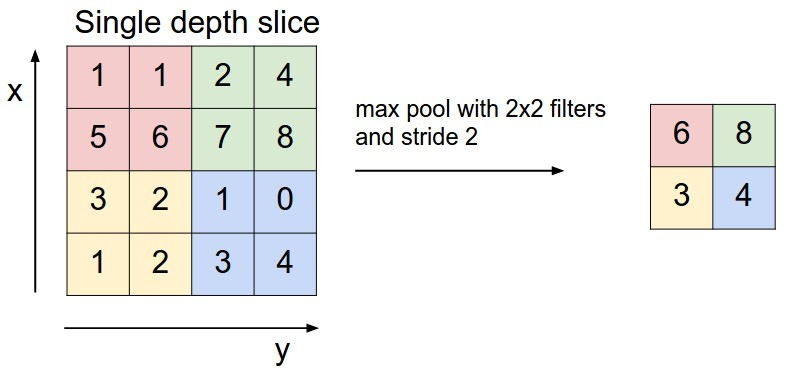
\includegraphics[width=0.7\linewidth]{maxpool.jpg}
  \caption[Max pooling]{
    Max pooling with a filter size of $2 \times 2$
    and stride $2$.
  }
  \label{fig:maxpool}
\end{figure}

\paragraph{}
Pooling reduces the spatial size
while retaining the depth
as the depth describes the amount of features.
The idea behind the concept
is that spatial location of a feature is less important
than the activation of the feature
(note again the importance of translation invariance),
along with the notion that features are most important
in relation to other features.
Pooling therefore preserves relative location of each feature.

\paragraph{}
Even though most convolutional networks
tended to have pooling layers,
if not occasionally in between convolutional layers
then often right after them,
in recent years in the literature
there has been a tendency to avoid pooling layers altogether.
\citeauthor{Springenberg2015}
(\citeyear{Springenberg2015})
suggest that pooling does not always improve performance
if the network already has enough capacity for the data at hand
and indeed advocate the use of convolutional layers
with larger strides
and even more convolutional layer
to make up for the loss in power.

\section{Recurrent Neural Networks}
\label{sec:rnn}
Some tasks are sequential in nature,
meaning one sample depends on a previous one,
rather than data being independently
drawn from some underlying distribution.
Typical problems include speech and written language.

Recurrent neural networks are especially suited
for these domains.
They process input sequences one step at a time,
maintaining hidden state which will then
affect future output.
% TODO ref
Recurrent networks are achieved
by introducing connections that form cycles.

\paragraph{}
It is no wonder this class of artificial neural networks
draws the eye of the reinforcement learner designer.
A problem with a pure Markov state space
has no need of a network useful for learning dependencies between different states,
since by definition every state on its own is sufficient enough of a representation
and includes all necesary past states in its description.
However, some conceivable reinforcement learning problems
are not Markovian
or are only made to be so
by supplying extra information to the system
such as derived state
(imagine angular velocity in the cart pole experiment).
Both kinds of problems
could still benefit from RNNs.

Recall also from section \ref{sub:pomdp}
the class of Partially Observable Markov Decision Procceses (POMDP).
These are processes that simply lack all required information in
at least some state descriptions.
As a result this is the class of problems that benefit most
from recurrent neural networks
and as a result are of special interest in this thesis.

\subsection{Building Blocks and Training}
\label{sub:building_blocks_and_training}
As Recurrent Neural Networks form a class of networks,
I will go over the general approach taken instead of a specific version.

Whereas regular feed-forward networks contain only forward connections,
RNN's usually contain cycles allowing them to capture time dependencies.
The cycle allows on state to depend on a previous one,
making it the ideal setup for sequences.

\begin{figure}[htpb]
  \centering
  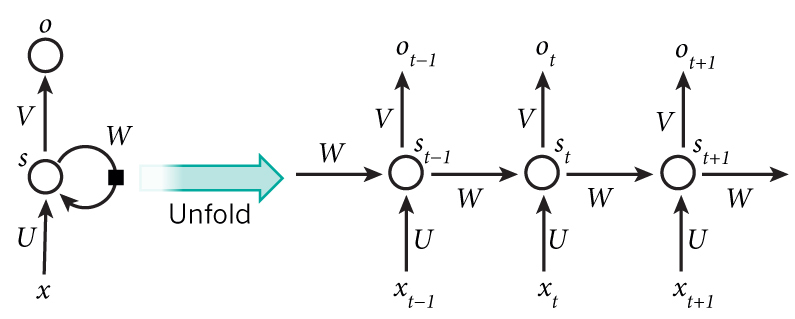
\includegraphics[width=0.8\linewidth]{rnn.jpg}
  \caption[Recurrent neural network time unfolding]{
    Recurrent Neural Network unfolded through time
    \parencite{Y.2015dl}.
  }
  \label{fig:rnn}
\end{figure}

At first, it might look daunting to train a network with recurrent connections
and as a result a recursive component in the error.
However, recurrent neural networks can simply be trained with gradient descent.
Figure \ref{fig:rnn} shows how a recurrent connection can be viewed
throughout three different time steps.
Seen in this rolled out fashion,
it simply becomes a very deep network with shared weights
and allows us to apply the well-known backpropagation algorithm.

\subsection{Long Short-Term Memory Networks}
\label{sec:lstm}
Regular recurrent neural networks can suffer from two problems during training:
\textit{vanishing gradient} and {exploding gradient}.
Highlighted first by
\citeauthor{hochreiter1991untersuchungen} (\citeyear{hochreiter1991untersuchungen})
and further characterized by
\citeauthor{bengio1994} (\citeyear{bengio1994}),
these two recurring problematic phenomena have long prevented
efficient traiffic of recurrent neural networks.

The \textit{exploding gradient} describes the norm of the gradient
increasing during training
because of explosive growth of the long-term components
which then far outweigh the short-term components.
The opposite phenomenon, \textit{vanishing gradient},
features more prominently in the literature.
It describes long term components that go exponentially fast to zero,
making it practically impossible to learn
long-term time dependencies of arbitrary length.

To deal with the exploding gradient,
\parencite{Pascanu2012}
suggest clipping the norm of the gradients
and
\citeauthor{Graves2013} (\citeyear{Graves2013})
show that \textit{skip connections},
i.e. connections that `skip' a layer,
help mitigate the vanishing gradient problem
for deep networks.

\paragraph{}
An architecture especially good at storing and accessing information
is the \textit{Long Short-Term Memory},
introduced by \citeauthor{Hochreiter1997} (\citeyear{Hochreiter1997}).
It remedies extreme gradients
by enforcing a constant error flow through special internal units.
It also contains gates that regulate
which inputs get remembered or even forgotten,
as well as gates that regulate when to output a remembered value.

\begin{figure}[htpb]
  \centering
  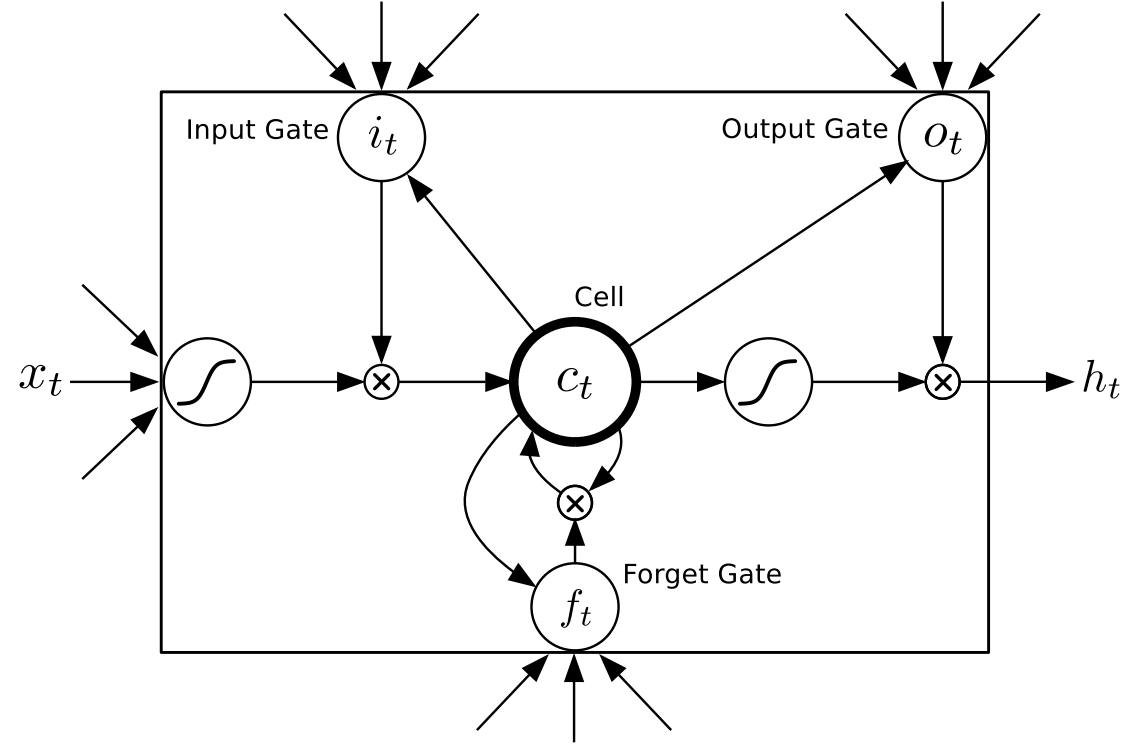
\includegraphics[width=0.8\linewidth]{lstm.png}
  \caption[Long Short-Term Memory]{
    Long Short-Term Memory cell
  \parencite{Graves2013}.
  }
  \label{fig:lstm}
\end{figure}

\paragraph{}
The basic unit is a Long Short-Term Memory cell
which is displayed schematically in Figure \ref{fig:lstm}.
A cell contains three gates:
an input gate, forget gate and output gate.
Each gate uses an activation function,
often the sigmoid function.
Central to it all is the cell unit, the internal state,
which gets regulated by the gates
in a fashion described by their names;
one gate controls whether the internal state should be overridden,
the other whether it should be used in the output
and yet another whether the internal state should be forgotten.
The combination of these elements make the LSTM cell into
into a veritable piece of memory.

\paragraph{}
Quite a lot of LSTM variants have been developed over the years
since their the LSTM's inception.
Below I describe the relations between the different components
as they are used in this thesis,
based on a popular design described by
\citeauthor{Graves2013} (\citeyear{Graves2013}).
Note that $\sigma$ is the sigmoid activation function
as described in section \ref{sec:sigmoid}.

\begin{align}
  &i_t = \sigma(W_{xi}x_t + W_{hi}h_{t-1}+W_{ci}c_{t-1} + b_i) \\
  &f_t = \sigma(W_{xf}x_t + W_{hf}h_{t-1}+W_{cf}c_{t-1} + b_f) \\
  &o_t = \sigma(W_{xo}x_t + W_{ho}h_{t-1}+W_{co}c_{t-1} + b_o) \\
  &c_t = f_tc_{t-1}+i_t tanh(W_{xc}x_t+W_{hc}h_{t-1}+b_c) \\
  &h_t = o_t tanh(c_t)
\end{align}

The $W_{ij}$ notation denotes the weights associated
with the connection from unit $i$ to unit $j$.
Likewise, $b_k$ denotes the bias for unit $k$.

While the equations might look daunting at first glance,
they can all be given intuitive meaning.
The three gates behave similarly;
they all depend on the current cell input ($x_t$),
the previous output ($h_{t-1}$)
and previous internal cell state ($c_{t-1}$).
All combine these inputs using a linear computation
and become non-linear through the activation function.
The connections from the previous cell state
to a gate are called \textit{peephole connections},
first introduced by
\citeauthor{gers2000recurrent} (\citeyear{gers2000recurrent}).

\paragraph{}
The internal cell state is a combination
of a `forget component' that determines
how the previous cell state is carried over
along with a combination of the current input and the previous output,
weighted by the current input gate
which regulates how the input should be used.

It must be noted that the original LSTM proposal
did not contain a forget gate
and simply added unchanged cell state
back into the current update.
This cell state was then referred to as the Constant Error Carousel (CEC),
named so because it enforced a constant error
in order to mitigate the vanishing and exploding gradient problems.


\section{Deep Q-Network}
\label{sec:dqn}
In \citeyear{Mnih2013},
\citeauthor{Mnih2013} at DeepMind
published a network
with raw pixels as input
that successfully
approached and even outperformed human ability
on a range of Atari 2600 games.
Two years later,
in \citeyear{Mnih2015},
\citeauthor{Mnih2015}
perfected the design of the network
which allowed it to be on par
and often outperform human players
on the majority of games considered.

Ever since,
extensions and
alternatives based on the same principles
have received a lot of attention.
One such a recent alternative is
Deep DPG
\parencite{Lillicrap2016}
which is an actor-critic approach
which learns a parameterized policy
instead of a value function.
Interesting extensions include
Prioritized Experience Replay
\parencite{Schaul2016}
which speeds up learning significantly
by making smarter use of stored experience
and
Deep Recurrent Q-Network
\parencite{Hausknecht2015}
which incorporates
a recurrent layer into its architecture.

\paragraph{}
This section is devoted to explaining why the Deep Q-Network
performed so well and what set it apart from previous attempts.
While there are two publications on the DQN architecture
(\citeyear{Mnih2013} and \citeyear{Mnih2015}),
the core as I explain it here is roughly the same;
they differ on a wide array of network parameters and learning parameters,
yet there are few structural differences.
When I use DQN in the text to follow,
I refer to the conceptual architecture that underlies both
except where noted explicitly.

\subsection{Problem Setting}
\label{sub:dqn_problem_setting}
The problem DQN attempts to solve
is that of a learning agent which finds itself playing an Atari game.
It does not know which game;
all it knows to be available to it
are consecutive observations of raw pixel values
and a scalar reward signal,
along with a number of unidentified actions it can take.
A more detailed investigation of this environment
can be found in section \ref{sec:ale}
where I describe the Arcade Learning Environment.

\paragraph{}
There are quite a few things that make the environment
challenging to a learning agent.
While the action space is small,
the state space is huge even though it is still finite.
This means tabulation variants of learning algorithms
are no longer feasible and function approximation must be employed instead.
This approximator used is a complex network,
the architecture of which is described further down.

\paragraph{}
Then there are a few difficulties
unique to the reinforcement learning problem.

The first is the \textit{credit assignment problem}:
given a reward,
how should the learner distribute credit to each of its previous actions
in a way that optimally reflects the impact of that action on the outcome.
Credit assignment is necessary and important
in order to distinguish between truly important actions
- game changers in this scenario maybe even -
and less important actions
that necessarily bridge the gap between crucial events.

The environment presented here features this problem
in varying degrees depending on the game in question
since some games can have a huge delay between
the reward and the core action or sequence of actions
that inevitably caused it.
The fact that this delay is very game-dependent
forms another challenge:
we want to be able to face all games with a uniform architecture.

\paragraph{}
Another issue is the need for good function approximation
while most techniques are tailored to the supervised learning setting
where data comes from a static distribution.
Since we update Q-values as we go
and indeed bootstrap updates with old values,
our target distribution is far from static and
is only expected to become stable
as the network converges.

Added to this is the fact that consecutive states
are highly correlated,
another characteristic that must be taken into account
when using learning algorithms
that assume independent data samples.

\subsection{Deep Q-Learning}
\label{sub:deep_q_learning}
To cope with the various problems presented above,
a learning algorithm was devised that beautifully combines
and improves on previous attempts to improve learning.

To start with,
while reinforcement learning is inherently online,
a technique called \textit{experience replay}
\parencite{lin1993}
is employed that allows us to combat some of the previously mentioned challenges.
An agent's experiences are stored in a data-set $\mathcal{D}$
as quadruples $e_t = (s_t, a_t, r_t, s_{t+1})$
at each time step $t$.
During the agent's experience gathering,
every few steps,
we apply a Q-learning minibatch update to a sample of the experience
$e \sim \mathcal{D}$
that is randomly drawn from the experience database.

Note that the use of experience replay condemns us to off-policy learning
because the policy has already changed at the time a sample is sampled.
The off-policy learning algorithm of choice for DQN
was Q-learning,
resulting in the complete \textit{Deep Q-Learning}
algorithm in listing \ref{algo:deep_q_learning}.

\paragraph{}
Another important addition to the algorithm
is the use of a separate network to generate target values
for Q-value updates.
Say the network is $Q$,
then at startup and every $C$ updates
we clone $Q$ to obtain $\hat{Q}$,
the target network that we will use to generate target Q-values
for the next $C$ updates.

This effectively makes the target distribution stable
for $C$ updates at a time.
Of course it still needs to change
but the frequency at which this happens
makes divergence unlikely.
An empirical indication of this behavior
is presented in Figure \ref{fig:freeze_qs}.

% TODO yeah I didn't really explain \phi, or eps, or rmsprop
\begin{algorithm}
  \caption{Deep Q-Learning with Experience Replay}
\label{algo:deep_q_learning}
\begin{algorithmic}
  \State Initialize replay memory $\mathcal{D}$ with capacity $N$
  \State Initialize action-value function $Q$ with random weights $\theta$
  \State Initialize $\hat{Q}$ with parameters $\theta'$ to a clone of $Q$
  \ForAll{episode}
    \State Initialize start state $s_1$ and processed observation $\phi_1 = \phi(s_1)$
    \For{$t=1, T$}
      \State With chance $\epsilon$ select random action $a_t$
      \State Otherwise select $a_t = \text{argmax}_a Q(\phi(s_t), a; \theta)$
      \State Perform action $a_t$, receive reward $r_t$ and observe $s_{t+1}$
      \State Store $(\phi_t, a_t, r_t, \phi(s_{t+1}))$ in $\mathcal{D}$
      \State Sample random minibatch $(\phi_j, a_j, r_j, \phi_{j+1})$ from $\mathcal{D}$
      \If{episode terminates at $j+1$}
        \State $y_j \gets r_j$
      \Else
      \State $y_j \gets r_j + \gamma max_{a'} \hat{Q}(\phi_{j+1}, a';\theta')$
      \EndIf
      \State Perform gradient descent step with error
      $(y_j-Q\left(\phi_j,a_j;\theta)\right)^2$
      w.r.t to the network parameters $\theta$
      \State Reset $\hat{Q} = Q$ every C steps
    \EndFor
  \EndFor
\end{algorithmic}
\end{algorithm}

\paragraph{}
Note that the replay memory is usually finite for practical reasons.
Different replacement algorithms can be used once it is full
but the standard way to go about it
would be to replace the oldest first
in a First In First Out approach.

\paragraph{}
The advantages of the Deep Q-Learning approach described here
can be summed up in the following points.

\begin{itemize}
  \item The random draw is intended to break up the correlation
    between consecutive samples.
    This reduces the variance between updates.
  \item Each experience can be reused
    in multiple updates which boosts efficiency
    because neural networks tend to learn slowly
    and in the supervised learning context often need multiple passes
    over the same data-set.

    This idea of experience reuse has been further capitalized on by
    \citeauthor{Schaul2016} who introduced
    \textit{prioritized replay} (\citeyear{Schaul2016})
    based on the earlier \textit{prioritized sweeping} \parencite{Moore1993}
    which prioritizes state updates according to associated change in value.
  \item Learning off-policy like this approach does
    avoids the pitfalls of self-reinforcing feedback loops
    where a training distribution can contain mostly samples
    that contain the maximizing action,
    a situation which would only propagate itself using on-policy learning.
    Such a loop is of course nefarious to exploration
    and can cause the learning to get stuck in a local minimum.
  \item Using a target network makes the learning process much more stable.
\end{itemize}

\subsection{Model Architecture}
\label{sub:model_architecture}

\begin{figure}[h]
\center
\begin{subfigure}[b]{.49\textwidth}
  \centering
  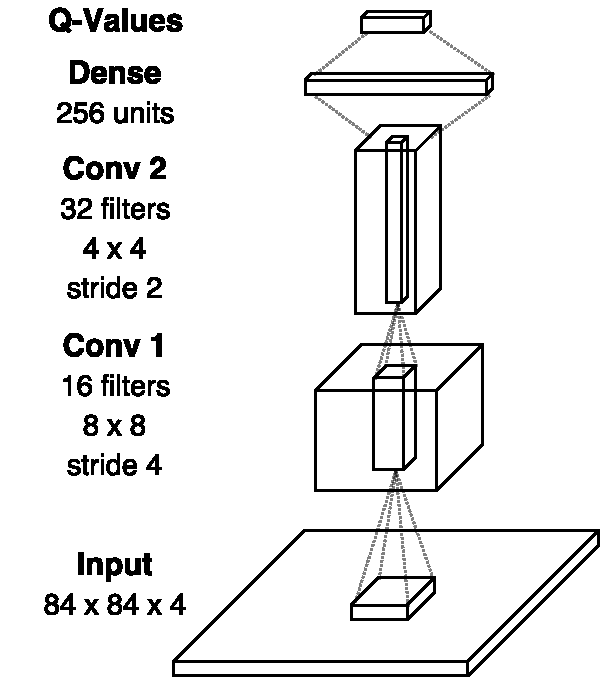
\includegraphics[width=\textwidth]{nips_network.pdf}
  \vspace{.1\baselineskip}
  \caption{Network described in \cite{Mnih2013}}
  \label{fig:nips_network}
\end{subfigure}
\begin{subfigure}[b]{.49\textwidth}
  \centering
  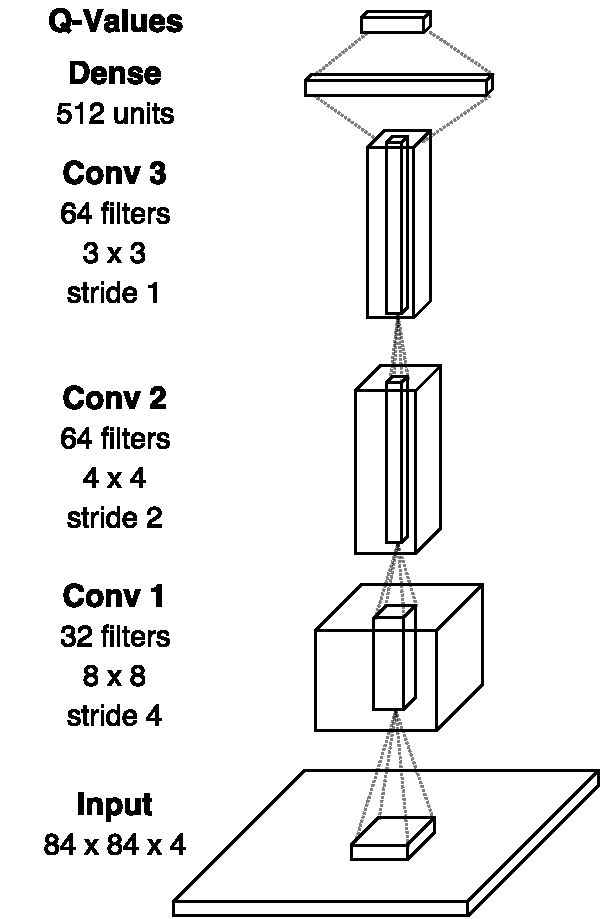
\includegraphics[width=\textwidth]{nature_network.pdf}
  \vspace{.1\baselineskip}
  \caption{Network described in \cite{Mnih2015}}
  \label{fig:nature_network}
\end{subfigure}
\caption[Original Deep Q-Networks]{
Two variations of the Deep Q-Network.
Both follow exactly the same principle
of stacking convolutional layers
that learn progressively more abstract features.
The inner area that is higlighted in each of the convolutional layers
illustrates how a single input tile is funnelled through the network
and gradually has more features learned on it,
demonstrated by the layers' increasing heights.
}
\label{fig:dqn_networks}
\end{figure}

Let us start by defining the input and output,
as DQN aims to be completely end-to-end.
There is still a preprocessing step to make training
the network more computationally feasible.
Atari frames are 210 x 160 pixels in size
with 7 bits for colors.
To vastly decrease the input space,
frames are processed to be 84 x 84.
The earlier paper simply cropped the image to
a region of the required size,
however the viability of this approach
is very game-dependent.
The later version scaled the image to the appropriate size.

Even though Atari colors nicely fit into a byte,
colors are converted to grayscale.

In order to make games Markovian or at least approximately so,
we use 4 image frames at a time,
which means two consecutive states
actually have 3 frames in common.
This proves to be sufficient for an agent to infer hidden features
like object velocities by inspecting the distance and direction
an object has travelled.
In next chapter I will go into a deeper discussion on this topic.
% TODO peter ref for 18 frames

The processing step described here corresponds to
the function $\phi$ in listing \ref{algo:deep_q_learning}.
Input to the network is now of size 84 x 84 x 4.
A 2D convolutional network can only cope with three dimensions:
two of which spatial and one for image depth,
or channels (an RGB image would have three).
This is interesting to note because the depth dimension
gets treated differently.

To illustrate without digging too much into the details,
number of image channels has no impact on the output shape of the
first convolutional layer as the new depth dimension size
of said output corresponds to the number of filters in the layer.
After the first convolutional layer,
there is nothing reminiscent in terms of shape
of the input depth.
Still, we have four frames at a time that we need to feed to the network.
DQN handles this by having only a single image channel
since everything is grayscale
and treats the time dimension as the image's channels.

\paragraph{}
Usually, when designing the Q function,
it would take as input a state and an action and produce
the corresponding Q-value.
In other words,
it would have the signature
$\mathcal{S} \times \mathcal{A} \mapsto \mathbb{R}$.
To get the action with the highest associated Q-value
for a certain state,
this function would then have to be evaluated
for each possible action.
While we only have a maximum of 18 actions,
the DQN approach is considerably more efficient
by computing the Q-values for all actions in a single forward pass.
The signature is now
$\mathcal{S} \mapsto \mathcal{A} \times \mathbb{R}$.
This means that the network will have an output unit
for each action whose value is the associated Q-value.

\paragraph{}
Now that we have a description
of both the input and output of the network,
we can start the discussion on the layers in between.
The two DQN architectures depicted in Figure \ref{fig:dqn_networks}
both follow the same concept
of stacking convolutional layers that
contain progressively more filters.
The first layer has the least amount of filters but uses the largest tiles
because it is meant for rougher low-level features,
of which there are suspected to be fewer than high-level ones.
The stride for each convolutional layer is set
to half the tile size for the first two layers,
so every tile overlaps up to four other tiles.
The overlap makes it so each pixel can have an impact
on multiple output units, spatially.

The output of each convolutional layer passes through a rectifier
nonlinearity \parencite{Nair2010}.

After the final convolutional layer
a single hidden fully connected layer is employed
which is meant to take full use of the features distilled
in the underlying convolutional layers.
The output layer is another fully connected layer
with the output of each unit corresponding to the q-value of an action
along with the input state.

There are a few differences between the two networks
depicted in Figure \ref{fig:dqn_networks}.
They all boil down to the same thing though:
representational power.
The network in Figure \ref{fig:nature_network}
has an extra convolutional layer
and each layer has more units than the corresponding one
in Figure \ref{fig:nips_network}.
More units mean the network has more raw capacity
but might take longer to train.

